\documentclass[letterpaper,12pt]{article}
\usepackage[section=2.1]{mathhw}

\usepackage{tikz}
\definecolor{bookblue}{RGB}{0, 173, 239}
\definecolor{bookgrey}{RGB}{219, 220, 222}

\begin{document}

\maketitle

\begin{enumerate}
  \item[1.]
    Four universities---1, 2, 3, and 4---are participating in a holiday basketball tournament. In the first round, 1 will play 2 and 3 will play 4. Then the two winners will play for the championship, and the two losers will also play. One possible outcome can be denoted by 1324 (1 beats 2 and 3 beats 4 in first-round games, and then 1 beats 3 and 2 beats 4).
    \begin{enumerate}
      \item[a.]
        List all outcomes in $\mathcal{S}$.
      \item[b.]
        Let $A$ denote the event that 1 wins the tournament. List outcomes in $A$.
      \item[c.]
        Let $B$ denote the event that 2 gets into the championship game. List outcomes in $B$.
      \item[d.]
        What are the outcomes in $A \cup B$ and in $A \cap B$? What are the outcomes in $A^\prime$?
    \end{enumerate}
  \item[2.]
    Suppose that vehicles taking a particular freeway exit can turn right ($R$), turn left ($L$), or go straight ($S$). Consider observing the direction for each of three successive vehicles.
    \begin{enumerate}
      \item[a.]
        List all outcomes in the event $A$ that all three vehicles go in the same direction.
      \item[b.]
        List all outcomes in the event $B$ that all three vehicles take different directions.
      \item[c.]
        List all outcomes in the event $C$ that exactly two of the three vehicles turn right.
      \item[d.]
        List all outcomes in the event $D$ that exactly two vehicles go in the same direction.
      \item[e.]
        List outcomes in $D^\prime$, $C \cup D$, and $C \cap D$.
    \end{enumerate}
  \item[3.]
    Three components are connected to form a system as shown in the accompanying diagram. Because the components in the 2–3 subsystem are connected in parallel, that subsystem will function if at least one of the two individual components functions. For the entire system to function, component 1 must function and so must the 2–3 subsystem.
    \begin{center}
      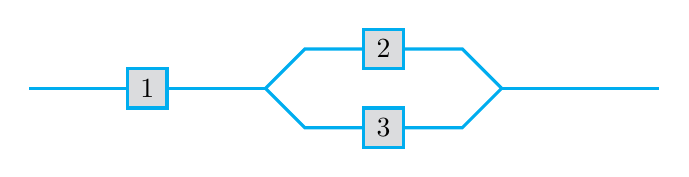
\begin{tikzpicture}[line width=0.4mm, draw=bookblue]
        \coordinate (A) at (3,0);
        \coordinate (B) at (3.5,0.5);
        \coordinate (C) at (5.5,0.5);
        \coordinate (D) at (6,0);
        \coordinate (E) at (5.5,-0.5);
        \coordinate (F) at (3.5,-0.5);

        \draw (0,0)--(A);
        \draw (A)--(B)--(C)--(D)--(E)--(F)--cycle;
        \draw (D)--(8,0);

        \filldraw[fill=bookgrey, draw=bookblue]
          (1.25,-0.25) rectangle (1.75,0.25)
          node[pos=.5] {1};

        \filldraw[fill=bookgrey, draw=bookblue]
          (4.25,0.25) rectangle (4.75,0.75)
          node[pos=.5] {2};

        \filldraw[fill=bookgrey, draw=bookblue]
          (4.25,-0.25) rectangle (4.75,-0.75)
          node[pos=.5] {3};
      \end{tikzpicture}
    \end{center}
    The experiment consists of determining the condition of each component [$S$ (success) for a functioning component and $F$ (failure) for a nonfunctioning component].
    \begin{enumerate}
      \item[a.]
        Which outcomes are contained in the event $A$ that exactly two out of the three components function?
      \item[b.]
        Which outcomes are contained in the event $B$ that at least two of the components function?
      \item[c.]
        Which outcomes are contained in the event $C$ that the system functions?
      \item[d.]
        List outcomes in $C^\prime$, $A \cup C$, $A \cap C$, $B \cup C$, and $B \cap C$.
    \end{enumerate}
  \item[8.]
    An engineering construction firm is currently working on power plants at three different sites. Let $A_i$ denote the event that the plant at site $i$ is completed by the contract date. Use the operations of union, intersection, and complementation to describe each of the following events in terms of $A_1$, $A_2$, and $A_3$, draw a Venn diagram, and shade the region corresponding to each one.
    \begin{enumerate}
      \item[a.]
        At least one plant is completed by the contract date.
      \item[b.]
        All plants are completed by the contract date.
      \item[c.]
        Only the plant at site 1 is completed by the contract date.
      \item[d.]
        Exactly one plant is completed by the contract date.
      \item[e.]
        Either the plant at site 1 or both of the other two plants are completed by the contract date.
    \end{enumerate}
\end{enumerate}

\end{document}
